Certains de vos enseignants mettront à votre disposition un carnet de classe. C'est un outil très pratique qui permet de prendre des notes et de modifier des fichiers mis à votre disposition, directement depuis Teams.

Pour accéder au carnet de classe, cliquez sur \textit{Bloc-notes de classe}, en haut de la page de la classe.

\begin{figure}[h]
	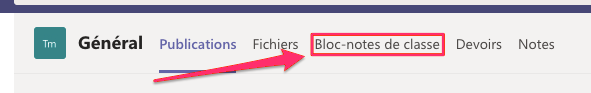
\includegraphics[width=9cm]{./images/bloc_notes/acces_bloc_notes_crop}
	\centering
\end{figure}

S'ouvre alors la page d'accueil du bloc-notes. Votre enseignant l'aura probablement adaptée à son cours, elle ne ressemblera donc pas forcément à l'image ci-dessous.

\begin{figure}[h]
	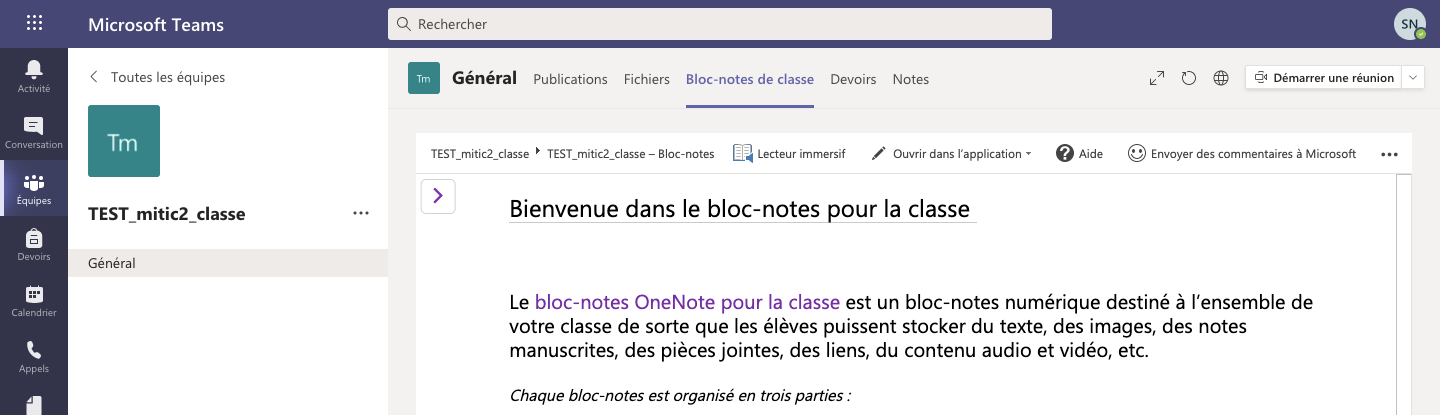
\includegraphics[width=11cm]{./images/bloc_notes/ouvrir_menu_bloc_notes_crop}
	\centering
\end{figure}

Cliquez sur la flèche en haut à gauche de l'espace de travail pour ouvrir la liste des bloc-notes. Une section à votre nom apparait, en bas de la liste. Il s'agit d'un espace personnel dans lequel vous pouvez écrire ce que vous voulez, que ce soit pour modifier des fichiers ou prendre des notes. Cliquez sur votre nom pour afficher des sous-sections.

\begin{figure}[h]
	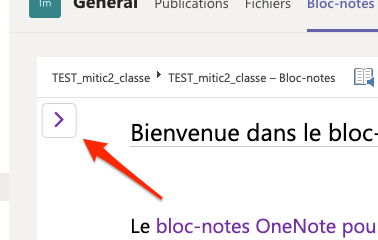
\includegraphics[width=6cm]{./images/bloc_notes/ouvrir_liste_dossiers_docs_crop}
	\centering
\end{figure}

Ouvrez la page sans titre, dans la sous-section \textit{Documents}. Ecrivez le titre de votre document. Vous verrez que le titre sera mis à jour dans la liste de documents, à gauche. Si votre liste de sections et documents s'est refermée, il suffit de cliquer sur la flèche, comme tout à l'heure, pour l'afficher à nouveau.

Vous pouvez maintenant écrire du texte, ajouter des images, ou modifier ce document comme vous le souhaitez.

Si vous souhaitez ajouter une nouvelle page, vous pouvez cliquer sur \textit{+ Page}, en bas. Renommez la nouvelle page en écrivant un titre comme vous venez de le faire.

\begin{figure}[h]
	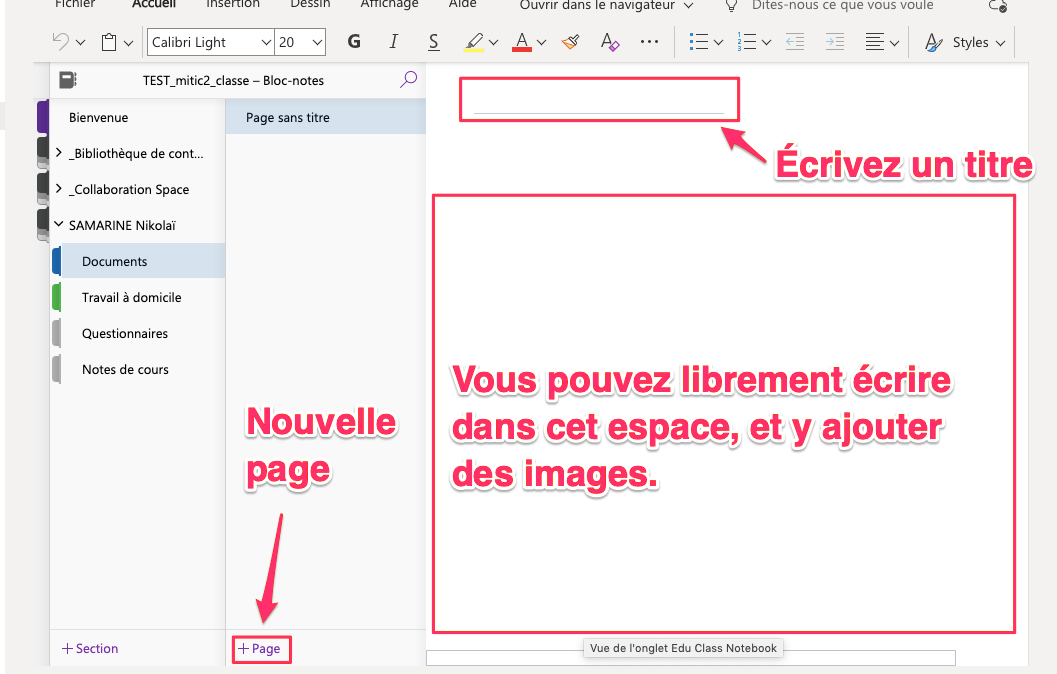
\includegraphics[width=10cm]{./images/bloc_notes/sous_section_documents_crop}
	\centering
\end{figure}

En ajoutant et modifiant ainsi des pages, vous allez pouvoir prendre des notes et y accéder via divers appareils, que ce soit depuis la maison ou l'école.